\documentclass[10pt,a4paper,twoside]{article}
\usepackage[utf8]{inputenc}
\usepackage{amsmath}
\usepackage{amsfonts}
\usepackage{amssymb}
\usepackage{graphicx}
\usepackage[left=2cm,right=2cm,top=2cm,bottom=2cm]{geometry}

%--------------------Phần package hình
\usepackage{tikz}
\usetikzlibrary{shapes.geometric, arrows, positioning,fit}

\tikzstyle{startstop1} =
[
	rectangle
	, text width=2cm
	, minimum height=0.8cm
	, text badly centered
	, draw=black
	, fill=white
]
\tikzstyle{process1}= 
[
	rectangle
	, text width=3.4cm
	, minimum height=0.8cm
	, draw=black
	, fill=white
]
\tikzstyle{process2}= 
[	
	rectangle
	, text width=2.5cm
	, minimum height=0.8cm
	, draw=black
	, fill=white
]
\tikzstyle{process3}=
[
	rectangle
	,rounded corners
	,minimum width=4cm
	,text height=0.35cm
	,draw=black
	,fill=white
	,text centered
]
\tikzstyle{process4}=
[
	rectangle
	,rounded corners
	,minimum width=4cm
	,text height=0.4cm
	,draw=black
	,fill=white
	,text centered
]
\tikzstyle{process5}=
[
	rectangle
	,minimum width=1.6cm
	,text height=0.5cm
	,text badly centered
	,draw=black
]
\tikzstyle{hinhthoi1}=
[
	diamond
	,text width=3cm
	,text height=0
	,text centered
	,draw=black
	,fill=white
] 
\tikzstyle{cloud}=
[
	draw
	,ellipse
	,fill=white
	,node distance=3cm
	,minimum height=1cm
	,text width=2cm
	,text centered
]
\tikzstyle{c}=
[	
	draw
	,text height=0.5cm
	,text width=3cm
	,cylinder
	,shape border rotate=90
	,shape aspect=0.2
	,text centered
]
\tikzstyle{binhhanh}=
[
	trapezium
	,trapezium left angle=70
	,trapezium right angle=110
	,text width=4cm
	,minimum height=1.5cm
	,draw=black
	,fill=white
]
\tikzstyle{khongvien}=
[
	rectangle
	,text centered
	,minimum width=0cm
	,minimum height=0cm
	,draw=white
	,fill=white
]

\tikzstyle{arrow} = [thick,->,>=stealth]
\tikzstyle{line} = [thick,-]


%--------------- Thanh ngang 
\usepackage{tikz}
%--------------- Chỉnh lại Header
\setlength{\headheight}{22pt}
%----------------
\usepackage{color}
\usepackage{framed}
\usepackage{fancyhdr}
\thispagestyle{empty} 
%------------------- Chia cột
\usepackage{multicol}

%-------------------Phần Header
\fancyhf{}
\rhead{\fontsize{8pt}{15pt}\selectfont \emph{ISSN (Print) : 0974-6846}\\
\vspace{-0,2cm}
\emph{ISSN (Online) : 0974-5645}}
\renewcommand{\headrulewidth}{0pt}
\lhead{\fontsize{6pt}{21.3096pt}\selectfont \textbf{Indian Journal of Science and Technology}, Vol 9(11), DOI: 10.17485/ijst/2016/v9i11/88460, March 2016}
\lfoot{} 
\thispagestyle{fancy}

%-------------------------Ngăn thụt đầu dòng
\setlength{\parindent}{0pt}
%-------------------------
\begin{document}
%-------------------------Định dạng màu
\definecolor{tieude}{rgb}{0,0.411,0.667}
%--------------------------
{\Huge \color{tieude}
\begin{flushright}
\fontsize{17,28pt}{23pt}\selectfont \LARGE{\textbf{Speech Emotion Recognition: Performance Analysis based on Fused Algorithms and GMM Modelling}}
\end{flushright}}
\begin{flushright}
\textbf{{R. Subhashree}$^1$ and {G. N. Rathna}$^2$}
\end{flushright}
%--------------------------
\begin{flushright}
{{$^1${Department of Electrical Engineering, Amrita University, Amritanagar Post, Ettimadai,}\\
Coimbatore - 641112, Tamil Nadu, India.\\
$^2$Department of Electrical Engineering, Indian Institute of Sciences, C V Raman Ave,\\
Bengaluru - 560012, Karnataka, India;\\
z-E-mail: subha94@ymail.com, rathna@ee.iisc.ernet.in}}
\end{flushright}
%--------------------------
\vspace{-0,4cm}
\begin{tikzpicture}[remember picture,overlay]
\path[left color=white,right color=blue]
([yshift=-215pt,xshift=8pt]current page.north west)
+(18.8,-0.05pt) rectangle +(1.5cm,0.05pt);
\end{tikzpicture}
%--------------------------Box 1
\setlength{\FrameRule}{2pt}
\setlength{\FrameSep}{5pt}
\definecolor{shadecolor}{rgb}{0.929,0.949,0.976}
\begin{shaded}
{\color{tieude}{\textbf{Abstract}}}\\
%-----------
\fontsize{9pt}{13pt}\selectfont
%-----------
\textbf{Background/Objectives:} Speech emotion recognition (SER) is an important aspect of Human-Computer Interaction systems which is widely used in different sectors like healthcare, robotics, automatic call centres and distance education.
Speech emotion recognition involves in depth analysis of the signal and identifying the appropriate emotion based on
its trained database using extracted features. \textbf{Method/Statistical Analysis:} This paper aims in devising SER system
using linear prediction of the causal part of the autocorrelation sequence (OSALPC) algorithm which has been proven
to efficiently reduce noise along with Linear Frequency Cepstral Coefficients (LFCC), Linear Predictive Coding (LPC),
MFCC, LPC using cepstrum for feature extraction. After extracting the feature vectors from the voice signal, it is modelled \textbf{Findings:}
Performance was analysed and our proposed system showed an overall efficiency of 89\% when tested on German database
(Emo-DB) for 7 emotions. The overall efficiency has proven to increase compared to the studies made up to date on the
German Database. The highest emotion recognition rate was for SAD using fused algorithm which was 95.56\%. Also results
were tabulated and compared using Modified MFCC. A Graphical unit interface of the proposed system is also devised.
\textbf{Application/Improvements:} The applications of speech emotion recognition are farfetched. Further scope of this work
will be a comparison of the achieved recognition rate using algorithms with recognition rate achieved by humans.
\end{shaded}
%-----------------------------------------
\vspace{-0,7cm}
{\color{tieude}\rule{17cm}{0,1pt}}\\
{\color{tieude}\textbf{Keywords:}} Emotion Recognition, LPC, MFCC, GMM, MAP, OSALPC
%--------------------------- Văn bản 1
\begin{multicols}{2}
%--------------------------Thanh ngang 1
{\Large  \color{tieude} \rmfamily \textbf{1. Introduction}}

\begin{tikzpicture}[remember picture,overlay]
\path[left color=gray,right color=white]
([yshift=-469pt,xshift=-0.5pt]current page.north west)
+(10.5,-0.1pt) rectangle +(2cm,0.5pt);
\end{tikzpicture}
{\vspace*{-1pt}
%-------------------------
\hspace*{-10pt} Recognizing emotions from speech had diverse appli
cations in different felds ranging from health care and
medicine to entertainment. Currently it is predomi
nantly being used for facilitating interaction of humans
with computers and robots. Such robots are used in
medicine for purposes like monitoring autistic people
and helping them interpret expressions and developing
a system for therapy and counselling, or in a brain-com
puter interface to interpret emotion from voice along
with facial expressions and EEG signals to help patients
deal with anxiety, stress and depression. It can also be
used in the feld of entertainment to identify the emo
tions and reactions of users. Various algorithms have
been deployed over the years for the two important pro
cesses involved in SER (Speech Emotion Recognition)
namely feature extraction and the decision making.
Some of the algorithms are Artifcial neural networks$^1$,
combination of linear prediction cepstrum coefcients
(LPCC), Mel Frequency cepstrum coefcients (MFCC),
Linear Prediction coefcients and Mel cepstrum coef
fcients (LPCMCC) and the Support Vector Machine
(SVM); combination of HMM and SVM, ANN, KNN,
MLBetc$^2$; MFCC, Discrete wavelet transforms with
SVM, Feature extraction algorithm based on Field}
\end{multicols}
{\color{tieude}\ \rule{3cm}{0.1pt}}\\
$^*$Author for correspondence
\begin{tikzpicture}[remember picture,overlay]
\path[left color=white,right color=blue]
([yshift=-39pt,xshift=8pt]current page.north west)
+(18.7,-0.2pt) rectangle +(1.75cm,0.5pt);
\end{tikzpicture}
%----------------------BẮT ĐẦU TRANG 2

\newpage
%----------------------Header 2
\pagestyle{fancy}
\fancyhf{}
\fancyhead[LE]
{\color{gray} \sffamily Speech Emotion Recognition: Performance Analysis based on Fused Algorithms and GMM Modelling}
\fancyhead[CE,CO]
{\begin{tikzpicture}[remember picture,overlay]
\path[left color=gray,right color=gray]
([yshift=-42pt,xshift=8pt]current page.north west)
+(18.7,-0.2pt) rectangle +(1.75cm,0.5pt);
\path[left color=gray,right color=gray]
([yshift=-45pt,xshift=8pt]current page.north west)
+(18.7,-2pt) rectangle +(1.75cm,0.5pt);
\end{tikzpicture}}
\fancyhead[RO]{R. Subhashree and G. N. Rathna}
\fancyfoot[LE,RO]{{\scriptsize \textbf{\thepage} \hspace{0.15cm} {\color{tieude} \textbf{\textbar}} \hspace{0.1cm}Vol 9 (11) \textbar \hspace{0.1cm} March 2016 \textbar \hspace{0.1cm} www.indjst.org}}
\fancyfoot[RE,LO]{{\scriptsize Indian Journal of Science and Technology}}
%----------------------

\begin{multicols*}{2}
programmable gate array$^3$ etc. For further insight into
state of the art of emotion recognition the following
can be referred$^4$. However, the real time application of
SER in noisy environment still remains unaddressed.
Our proposed system tries to deploy a combination of
fve algorithms for feature extraction namely MFCC,
LPC, LPCC, LFCC and OSALPC to devise emotion
recognition system in noisy environment by tabulating the results for different input noise levels. OSALPC
which is a proven algorithm for high efciency in noisy
environments, has till date been used only for speech
recognition$^5$. Tis paper proves the effectiveness of
OSALPC in emotion recognition.
\smallskip

\begin{tikzpicture}[remember picture,overlay]
\path[left color=gray,right color=white]
([yshift=-250pt,xshift=8pt]current page.north west)
+(10.5,-0.1pt) rectangle +(1.7cm,0.5pt);
\end{tikzpicture}
{\Large  \color{tieude} \rmfamily \textbf{2. Proposed System }}

\section*{\color{tieude} {\fontsize{11pt}{13pt}\selectfont 2.1 Data Set}}

Tests were conducted on an authentic Data Set
EMO-DB6, a German data base. Around 200 voices were
recorded from the Database. Tese fles were sampled
at 16000Hz and converted to wav fles in Matlab. Te
data base consists of voice samples of 7 emotions spoken
by 10 trained artists of both genders and different ages. Te recordings are for 10 sentences spoken in German.
Te 7 emotions are happy, sad, angry, disgust, fear, boredom and neutral. Te overall flow chart of the proposed
system is given in Figure 1.
\smallskip
\section*{\color{tieude} {\fontsize{11pt}{13pt}\selectfont 2.2 Pre-Processing}}

Speech signals are normally pre-processed before feature extraction to mainly boost the amount of energy
in the higher frequencies with respect to lower frequencies.\\
This is also known as pre-emphasis$^7$. We have used the
following flter.
\begin{center}
%% công thức 2
$
Y(n)=X(n)-0.97\text{\raisebox{0.9ex}{\mbox{\scriptsize$\star$}}}X(n-1)
$
\end{center}
\section*{\color{tieude} {\fontsize{11pt}{13pt}\selectfont 2.3 Pre-Emphasis}}

Initially, fltering technique is applied to reduce the noise
and optimize the classifcation of features using a high
pass flter.\\
Framing is then done to convert audio signals into
frames of overlapping blocks. Each frame consists of 200
samples of data and obtained from voice fles.
\columnbreak

%--------------------- Hình " Figure 1. Overall flowchart. "
\begin{tikzpicture}[node distance=2.5cm]
\node(start)[cloud]{ START};
\node(pro) [process1,below of=start,text width=7cm,text height=2.3cm,text centered]  {\bfseries{\raisebox{0cm}{GERMAN DATA BASE(EMO-DB)}}}  ;
\node(c)[c,below of=start,yshift=0.1cm]{\Large Dataset};
\node(pro1)[process5, below of=pro,xshift=-3.5cm,node distance=3.5cm]{MFCC};
\node(pro2)[process5, below of=pro, xshift=-1.5cm, node distance=3.5cm]{LFCC};
\node(pro3)[process5, below of=pro, xshift=0.5cm, node distance=3.5cm]{OSALPC};
\node(pro4)[process5, below of=pro, xshift=2.5cm, node distance=3.5cm]{LPC};
\node(pro5)[process5, below of=pro, xshift=4.5cm, node distance=3.5cm]{LPCC};
\node(vohinh1)[khongvien, below of=pro, node distance=2.5cm]{};
\node(vohinh2)[khongvien, below of=pro3,xshift=-1cm, node distance=1.5cm]{};
\node(bh1)[binhhanh,below of=vohinh2, node distance=1.5cm]{MAP CLASSIFIER \\ (MAXIMUM\\ A POSTERIORI)};
\node(bh2)[binhhanh, below of=bh1, node distance=2.5cm,text width=2cm, minimum height=2cm]{DETECTION UNIT AND COMBINED RESULT};
\node(end)[cloud,below of=bh2,node distance=2cm]{END};

\draw[arrow](start)--(pro);
\draw[arrow](pro.south)--(vohinh1);
\draw[arrow](vohinh1.north)-|(pro1);
\draw[arrow](vohinh1.north)-|(pro2);
\draw[arrow](vohinh1.north)-|(pro3);
\draw[arrow](vohinh1.north)-|(pro4);
\draw[arrow](vohinh1.north)-|(pro5);

\draw[line](pro1)|-(vohinh2.north);
\draw[line](pro2)|-(vohinh2.north);
\draw[line](pro3)|-(vohinh2.north);
\draw[line](pro4)|-(vohinh2.north);
\draw[line](pro5)|-(vohinh2.north);

\draw[arrow](bh1)--(bh2);
\draw[arrow](bh2)--(end);

\draw[arrow](vohinh2.north)--(bh1);

\end{tikzpicture}

\vspace*{0.25cm}
{\color{tieude} \textbf{Figure 1.}} Overall flowchart.

\section*{\color{tieude} {\fontsize{11pt}{13pt}\selectfont 2.4 Windowing}}

Tis windowing function weights the signal in the time
domain and divides it into a sequence of partial signals.
Hamming window is used to reduce the spectral leakage
in the input data signal. Te corresponding signals before
and afer pre-processing are given in Figure 2 and Figure 3.

\section*{\color{tieude} {\fontsize{11pt}{13pt}\selectfont 2.5 Feature Extraction Algorithms}}
\vspace{1cm}

{\color{tieude} \textbf{2.5.1 MFCC (Mel Frequency Cepstral
Coefcient) Algorithm}}
\bigskip

Te shape of the vocal tract, which determines what sound
comes out, manifests itself in the envelope of the short
time power spectrum of the speech signal and MFCCs
accurately represent this envelope. It has been proven
that the sensitivity of human ears to different frequency
\newpage
\hspace{0.5cm} \includegraphics[scale=1]{figure2}
{\color{\textbf{tieude} Figure 2.}} Signal before pre-processing.}
\end{multicols*}{2}
\end{document}
